\chapter{Desenvolvimento do Jogo}\label{ch:Desenvolvimento}

%A documentação do jogo é o Game Design Document (ou GDD para os íntimos). Alguns chamam também de Game Design Bible. É a mesma coisa

O processo de desenvolvimento de jogos digitais é uma tarefa que exige do(s) desenvolvedor(es) conhecimentos de programação. Um jogo para ser desenvolvido, deve ser escrito em uma determinada linguagem de programação, o que acaba por obrigar que o(s) desenvolver(es) do jogo tenha(m) conhecimento sobre esta linguagem. Embora existam linguagens de programação visual, o conhecimento sobre lógica de programação ainda é parte fundamental e essencial para o desenvolvimento de um jogo. 

%(programação em blocos ou Visual Scripting) : linguagem de programação visual. 

Um jogo digital requer conhecimentos computacionais específicos para o seu desenvolvimento. Aspectos técnicos e metodológicos devem ser levados em consideração durante todo o ciclo de desenvolvimento de um jogo. A \autoref{sec:Engenharia} trás fundamentação teórica detalhada a respeito dos principais aspectos metodológicos que tangem o jogo desenvolvido pela presente pesquisa. Brevemente, informa-se que o jogo digital, desenvolvido pelo corrente trabalho acadêmico, segue a metologia para o desenvolvido de jogos denominada de \textit{GAMED} \cite{aslan2016digital}. 

Definir uma metodologia de desenvolvido é essencial para se gerenciar melhor os prazos e recursos necessários de um projeto. Dada a importância dessa etapa, é crucial que a escolha da mesma esteja devidamente fundamentada. Por tal razão, que a metologia escolhida para guiar essa pesquisa é descrita no Capítulo de Fundamentação do presente trabalho acadêmico. Sendo assim, resta ao presente Capítulo, apresentar demais aspectos importantes que tange o jogo educaciol desenvolvido pela corrente pesquisa. No entanto, é essencial salientar aqui que, embora aspectos artísticos, sonoros, ergonômicos e jurídicos sejam importantes no desenvolvimento de jogos, eles não são abordados neste trabalho, assim como questões sobre usabilidade, acessibilidade, escalabilidade, flexibilidade, criptografia e segurança de dados.



O presente Capítulo apresenta as características gerais do jogo desenvolvido. Nesse sentido, tanto aspectos computacionais, quanto aspectos pedagógicos e metodológicos de ensino são descritos. Sendo assim, a \autoref{sec:motor} descreve as princpais caraterísticas gerais que tange o jogo desenvolvido por essa pesquisa, listando aspectos técnicos, tais como, dinâmicas e mecânicas utilizadas no jogo. A forma como essa mecânicas e dinâmicas interagem com os conceitos didáticos do jogo é descrita na \autoref{sec:DN}. Por fim, \autoref{sec:fim} dá as considerações finais do presente capítulo. 



%Além disso, para a confecção do jogo em tempo hábil uma metodologia deve ser seguida 

\begin{comment}
Métodologia 
Motor de jogo (ferramenta)
aspectos tecnicos:
publico alvo
plataforma
(BASEADO: infancia segura)
Escalabilidade/flexibilidade
Ergonomia
Estética = 2D isométrico
estilo = aventura
engajamento?
\end{comment}

%http://dualiby.com/adobet4t/gamification/imgs/gamedesign_canvas_pb.jpg

%O fato é que a mecânica do jogo (conjunto de regras e objetivos)

%Embora importantes no cenário de desenvolvimentos de jogos, aspectos artísticos, sonoros, ergonomicos, estéticos, aspectos jurídicos. 

%criptografia, banco de dados,

%demais aspectos de correspondem a infraestrutura não serão abordadaos. 


\section{Características Gerais}\label{sec:motor}

A presente pesquisa realiza o desenvolvimento de um jogo sério. O jogo em questão, baseia-se nas ideias propostas por \citeonline{diocesano2018infancia}. Visando apresentar as principais caractéristicas que definem o jogo sério produzido, confeccionou-se um \textit{Game Design Canvas} (GDC). A \autoref{fig:canvas} ilustra o \textit{Game Design Canvas} do jogo elaborado pelo atual trabalho acadêmico. 
%Game Design Canvas (GDC) é um framework para rapidamente definir os elementos fundamentais de um jogo \cite{sarinho2017proposta}


\vspace{-0.1cm}

\begin{figure}[hbt!]
  \caption{\label{fig:canvas}\textit{Game Design Canvas}}\vspace{-0.45cm}
  \begin{center}
    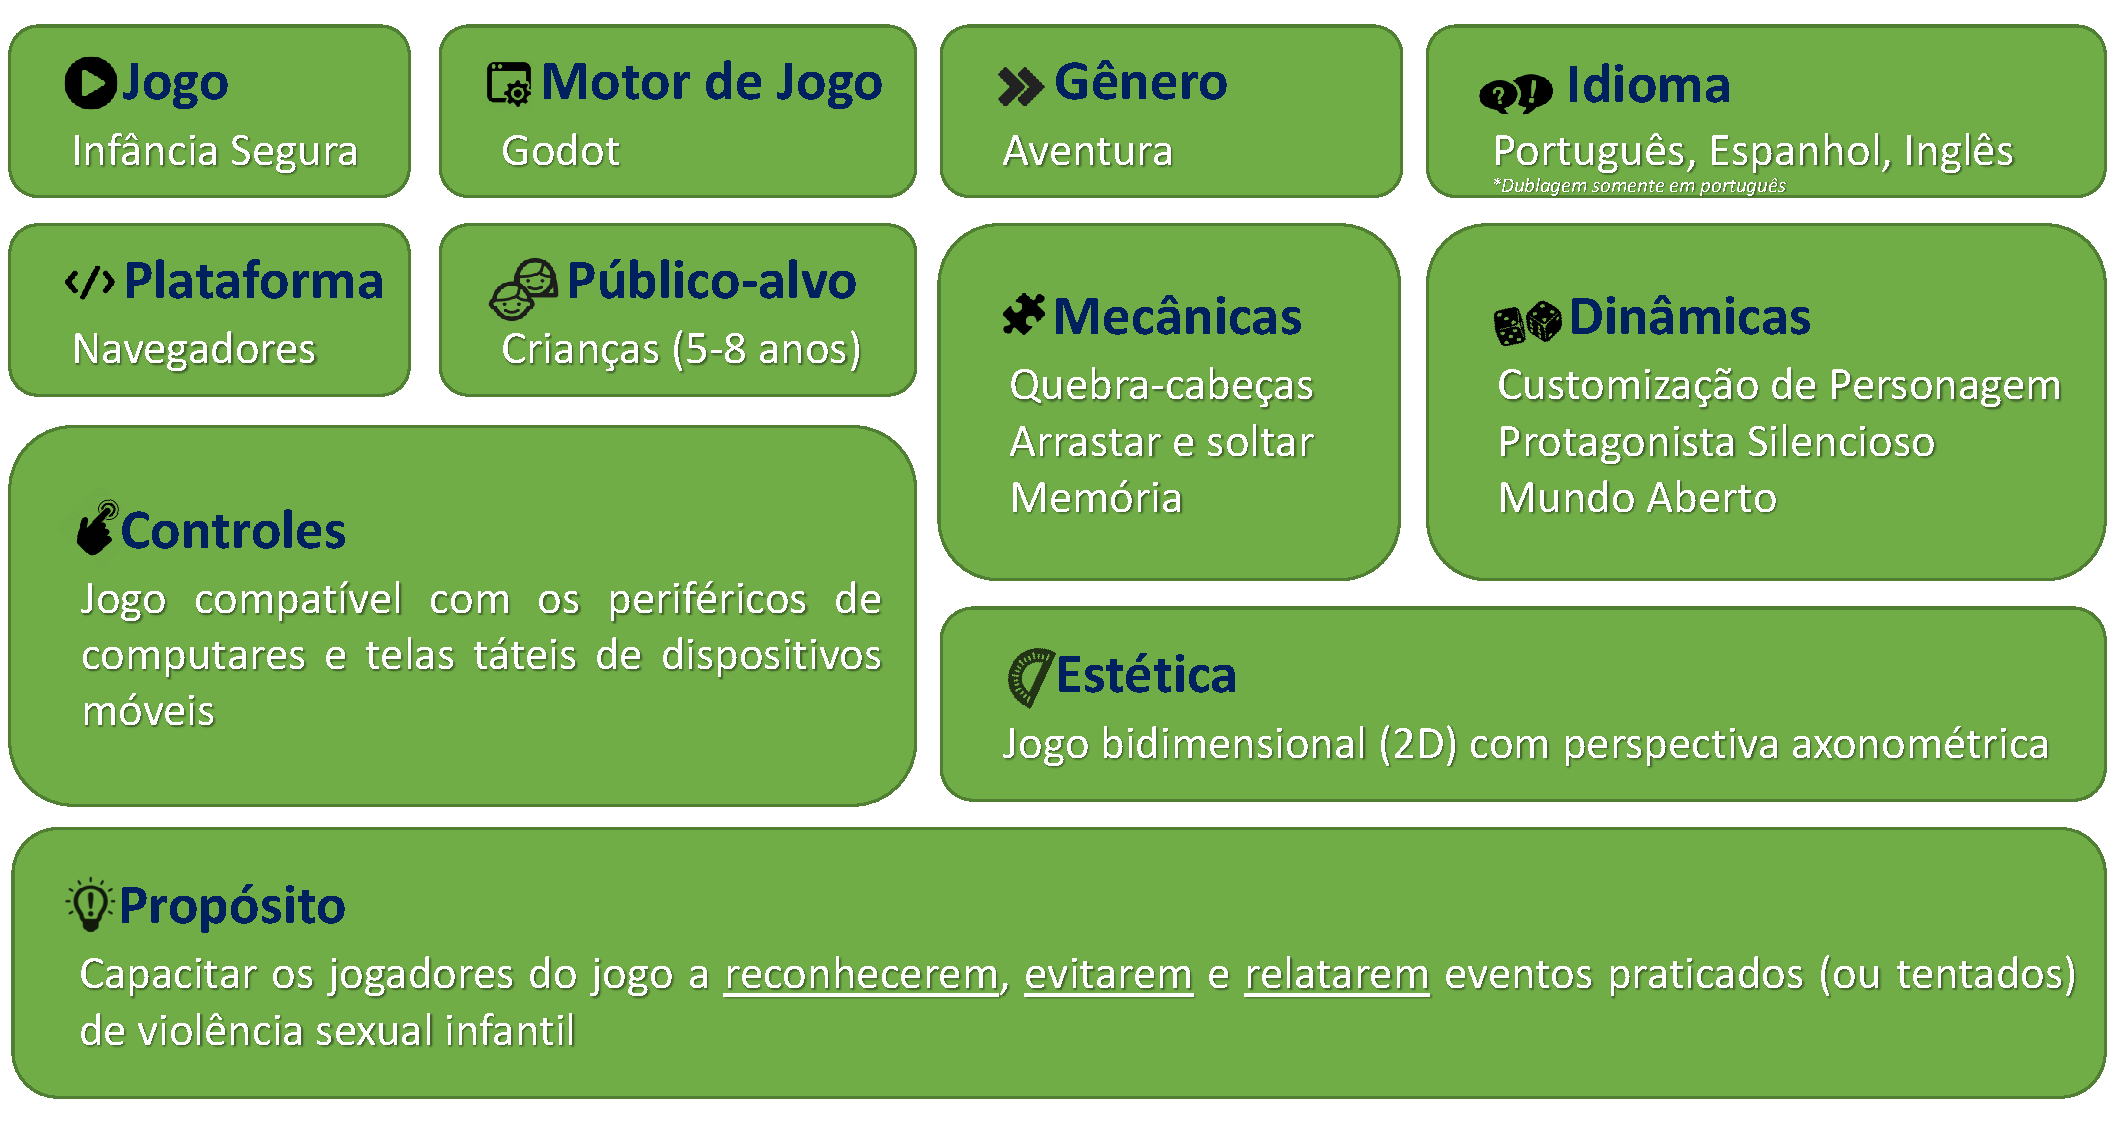
\includegraphics[width=\linewidth]{./Figuras/canvas.pdf}
    \end{center}\vspace{-0.8cm}
  \legend{Fonte: os autores}
\end{figure}

\vspace{-0.2cm}

A \autoref{fig:canvas} define as principais características do jogo desenvolvido. O jogo confecionado pelo correte trabalho herda algumas ideias propostas por \citeonline{diocesano2018infancia}, enquanto descarta outras (e.g. o jogo original baseia-se em um dinâmica linear de exploranção, ao invés de uma dinâmica de mundo aberto). Dentre os principais legados do jogo original estão: o nome do jogo, seu propósito, público-alvo e plataforma. O jogo denomina-se \textbf{Infância Segura}. Seu propósito consiste em desenvolver e aprimorar habilidades e conhecimentos específicos que viabilizem aos jogadores reconhecerem, evitarem e relatarem epsódios praticados (ou tentados) de violência sexual infantil. Para atingir a classe infantil, definiu-se um público-alvo de crianças entre cinco e oito anos. Essa idade é estabelecida com base nos conteúdos pedagogicos abordados pelo jogo, sendo conteúdos adequados a essa faixa etária de acordo com as orientações técnicas internacionais de educação em sexualidade da \citeonline{women2018international}. Buscando atingir um maior número de crianças, escolheu-se portar o jogo para navegadores, o que proporciona o jogo esteja disponivel a uma variedade maior de dispositos com o mínimo de alterações ou adpatações no código-fonte \cite{carrara2018criancca}. Essa escolha, faz com que os controles do jogo sejam compactíveis aos periférios dos computadores e as telas táteis dos dispositivos móveis. 


%A escolha de plataforma de navegadores, viabiliza o jogo esteja disponivel a uma variedade maior de dispositos com o mínimo de alterações ou adpatações no código-fonte \cite{carrara2018criancca}. Por tal razão que os controles do jogo são compactiveis aos periférios dos computadores e as telas táteis dos dispositivos móveis. 


%O jogo deve ser mediado por professores ou responsaveis/pais (denominados, aqui, educadores), de maneira que esses sejam ´ responsaveis por avaliar o n ´ umero de respostas certas/incorretas


O jogo desenvolvimento possui uma estética inteiramente bidimensional (2D), com perspetiva axonométrica. A bidimensionalidade do jogo agiliza o processo de desenvolvimento. A remoção uma dimensão do jogo, simplifica as etapas de programação e elaboração de cenários. Entretanto, jogos bidimensionais tendem a limitar a locomoção do personagem do jogador justamento por removerem uma dimensão. Para contornar isso, surgem os jogos em perspectiva axonométrica. Jogo axométricos, são jogos bidimensionais que não limitam a movimentação dos jogadores, permitindo que os mesmo possam locomover seus personagens tridimensionalmente em todo o cenário do jogo. 


%Ainda, buscando trazer maior agradabilidade aos jogadores, salienta-se que o jogo é inteiramente bidimensional (2D), no entanto com perspetiva axonométrica. A perspectiva axonométrica, permite que jogos possam ser desenvolvidos em duas dimensões (o que agiliza o processo desenvolvimento pois remove uma dimensão), sem limitar a locomoção e movimentação dos jogadores, permitindo que os mesmo possam se movimentar seus personagens tridimensionalmente no cenário do jogo.

Para que o cenário e todos os demais aspectos do jogo sejam mais compreensiveis aos jogadores é essencial promover algum mecanismo que facilite o aprendizado sobre seu funcionamento. Por tal razão, mediadores são fundamentais nos primeiros momentos de uso de um jogo, pois auxiliam o processo de compreensão das regras e da estrutura do jogo os jogadores. Todavia, nem sempre é possível ter mediadores para orientar os jogadores. Nestes casos, a implantação de um tutorial surge como forma de contornar esse problema, substituindo a presença de um mediador \cite{buchinger2014sherlock}. Um sistema de tutorial consite na ideia de  ensinar ao jogador como funcionam as dinâmicas de um jogo, apresentando as regras e as ações que o jogador pode exercer. Existem diversos meios para ensinar isso aos jogadores. No caso do jogo desenvolvido, o sistema de tutorial utilizado baseia-se na ideia de um tutor virtual que acompanha o jogador durante todo o jogo. O tutor virtual acompanha o personagem do jogador sem se distanciar muito. Isso é feito para reforçar os ensinamentos de que uma criança deve estar sempre acompanhada. %, além disso, espera-se que tal funcionalidade traga um sentimento de companheirismo ao jogador.
Junto a este sistema de ajuda ao jogador, também é implementado a dinâmica do herói mudo. %ou dinâmica do protagonista silencioso.

%Para que um game seja completo, e atenda a critérios de usabilidade, é essencial promover algum mecanismo que facilite o aprendizado do funcionamento do jogo. POr tal razão, mediadores são fundamentais nos primeiros dias, ou horas de uso de um jogo, porque eles podem ajudar a entender e orientar os jogadores \cite{buchinger2014sherlock}.Todavia, não é em todos os casos que é possível ter mediadores para orientar os jogadores. Nestes casos, a implantação de um tutorial parece ser essencial para, de certa forma, substituir a presença de um mediador. O aspecto principal de um tutorial é ensinar ao jogador como funcionam as dinâmicas de um jogo, apresentando as regras e o controle que o jogador pode exercer. Existem diversos meios para ensinar isso aos jogadores. No caso do jogo desenvolvido, isso é realizado através de um um tutor virtual que se manifesta na forma de uma criança. O personsagem tutor, além disso, acompanha o jogador durante todo o jogo O tutor virtual acompanha o personagem do jogador sem se distanciar muito. Isso ´e feito para refor¸car os ensinamentos de que uma crian¸ca deve estar sempre acompanhada, al´em disso, com tal funcionalidade espera-se trazer um sentimento de companheirismo ao jogador.




%O jogo desenvolvido por este trabalho permite a customização de personagem. Esse recurso gera um elo entre personagem e jogador, proporcionando que o jogador possa se sentir representado no jogo. Além disso, o jogo possui um sistema de tutorial baseado em um personagem que acompanha o jogador. Esse sistema de ajuda ao jogador é implementado para facilitar o aprendizado sobre o jogo e suas dinâmicas \cite{buchinger2014sherlock}. Junto a este sistema de ajuda ao jogador, também é implementado a dinâmica do herói mudo ou dinâmica do protagonista silencioso.


A dinâmica do herói mudo (ou protagonista silencioso) permite uma imersão maior ao jogador. Nessa dinâmica, o personagem do jogador não se expressa de maneira verbal \cite{domsch2017dialogue}. Graças a isso, não há o risco do personagem do jogador se utilizar de palavras ou de elementos contextuais que o jogador desconheça, proporcionando assim, uma conexão maior entre personagem e jogador. Como artifício, para dar enredo a história do jogo, as frases são transferidas para um personagem que o jogador não possui controle (o personagem tutor no presente jogo), com o intuito de evitar assim, uma disrupção da interligação entre personagem e jogador. Embora o personagem do jogador não fale; todos os diálogos do jogo são transcritos textualmente e verbalmente. A depender da configuração do jogo, os dialogos podem ser exibidos em português, espanhol, ou inglês. No entando, a verbalização dos dialógios (dublagem), encontra-se disponível somente em portugues. A dublagem associada ao texto escrito proporciona acessibilidade do jogo as crianças (falantes de português) que não se encontram plenamente alfabetizadas \cite{limeira2015avaliaccao}. 


%A prática de protagonistas silenciosos era utilizada no princípio do desenvolvimento de jogos devido a limitações tecnológicas, posteriormente se fez presente em histórias simples que não requeriam diálogo para narrar seus acontecimentos \cite{domsch2017dialogue}. Com a evolução da tecnologia, as empresas optaram em trazer um maior realismo aos jogos, no entanto a dinâmica do herói mudo permite uma imersão maior ao jogador, pois permite uma conexão maior entre personagem e jogador, uma vez que não há o risco do personagem se utilizar de palavras ou de elementos contextuais que o usuário desconheça. Nesse sentido, as perguntas são transferidas para um personagem que o jogador não possui controle (o personagem tutor), com o intuito de evitar assim, uma disrupção da interligação entre personagem e jogador.


O jogo para prevenção da violência sexual infantil projetado neste trabalho é do gênero aventura. Os jogos de aventura são jogos em que o jogador assume o papel de um protagonista em uma história interativa com exploração e resolução de quebra-cabeças. Os quebra-cabeças do presente jogo se traduzem em minijogos voltados a prevenção da violência sexual infantil. Ao se tratar do público infantil, observou-se que o gênero aventura, se destaca como o gênero de jogo que mais agrada de forma igualitária, meninos e meninas \cite{brandtzaeg2009children}. %tudo bem que são criança do norte da europa, maz fazer o que :P

Existem majoritaria dois caminhos que tangem o desenvolvimento e produção de jogos. Um jogo pode ser produzido em uma linguagem de programação, seguindo os protocolos e estruturas específicas de um determinado dispositivo, ou pode ser produzido sob um motor de jogo (\textit{Game Engine}). %No caso, motor de jogo é o nome dado a qualquer plataforma voltada para o desenvolvimento de jogos. 
Os motores de jogos proporcionam um ambiente completo para a criação de jogos, com toda a parte gráfica e sonora já abstraídas. Isso permite ao desenvolvedor exportar o jogo para diferentes sistemas computacionais realizando alterações mínimas no código-fonte \cite{bishop1998designing, machado2009serious}. 

Existem vários motores voltados para o desenvolvimento de jogos. O motor optado por este trabalho é o \textit{Godot}\footnote{\textit{Godot} é um motor de jogos totalmente gratuito e de código aberto sob a licença permissiva do MIT. O motor pode ser adquirido por meio do seguinte endereço: \url{https://godotengine.org/}.} (versão 3.2). Em comparação aos demais motores de jogos, o \textit{Godot} se destaca por ser totalmente gratuito, adaptado ao idioma português e por exportar os jogos para múltiplos sistemas \cite{scherer2020analise}. Salienta-se que a última versão estável da plataforma \textit{Godot} é a versão 3.2. Por tal razão essa é a versão que fundamenta as bases e o andamento do corrente trabalho acadêmico. 



Embora a plataforma exporte seus jogos para múltiplos sistemas, é importante destacar que o jogo desenvolvido neste trabalho está exportado apenas para navegadores. Fica a cargo de pesquisa futuras a adaptação do código-fonte para portar o jogo para difentes sistemas operacionais, possibilitando assim, que o jogo possa ser baixado e executado sem necessidade de uma conexão constante com os servidores. Em adendo, salienta-se que a atual versão do jogo salva as inforamções de desempenho dos jogadores em um banco de dados, toda vez que uma data etapa do jogo é finalizada. O registro dos dados dos jogadores é uma herança do jogo proposto por \citeonline{diocesano2018infancia}. Salienta-se no entando, que os dados não são filtrados ou tratados, sendo acessiveis somente através de requisições \textit{PHP}. Cabe então a pesquisa futura, a confecção de uma plataforma mais agradável de acesso a essas informações, forncendo visualização mais clara e precisa no que diz respeito ao desempenho dos jogadores, à professores ou responsvéis.


%Todo o processo de desenvolvimento do jogo ocorre em ambinete Linux, as linguagem utilizadas durante o processo de desenvolvimento são as liguagem ofertadas pelo Godot (C, C++), além de SQL e PHP para o gerenciamento e organização das informações em um banco de dados. 

\newpage




%\section{Ensinamento}\label{sec:ensinamento}

%Os participantes devem ser capazes de identificar corretamente a localização e o nome das partes do corpo.

%As crianças devem saber diferenciar as partes íntimas do corpo das demais partes. 

%Os participantes devem manifestar competências sobre o uso seguro das tecnologias da informação e comunicação.

%As crianças devem saber reconhecer um adulto em quem possam confiar.

\section{Desenho de Níveis e Ensinamentos}\label{sec:DN}



\begin{comment}

Com o objetivo de abstrair e elucidar melhor alguns conceitos do jogo formulou-se o diagrama de atividades do jogo, representado na \autoref{fig:Diagrama}. Um diagrama de atividade é essencialmente um fluxograma que mostra as atividades executadas por um sistema. Tradicionalmente em diagramas, o início de um processo é representado por um círculo preenchido; o final de um processo é representado por um círculo preenchido dentro de outro círculo; os retângulos com cantos arredondados representam atividades que devem ser realizadas; as setas representam a passagem de uma atividade para outra; o losango representa uma decisão; o paralelogramo representa a inserção de informações; o cilindro representa o banco de dados; o retângulo esticado representa a junção de atividades; o retângulo com linhas internas representa o armazenamento interno; o semi-retângulo circular representa um tempo de espera; e o pseudo-triângulo invertido representa uma atividade externa a aplicação.





\begin{figure}[hbt!]
\caption{\label{fig:Diagrama}Diagrama de Atividades do Jogo}\vspace{-0.4cm}
\begin{center}
  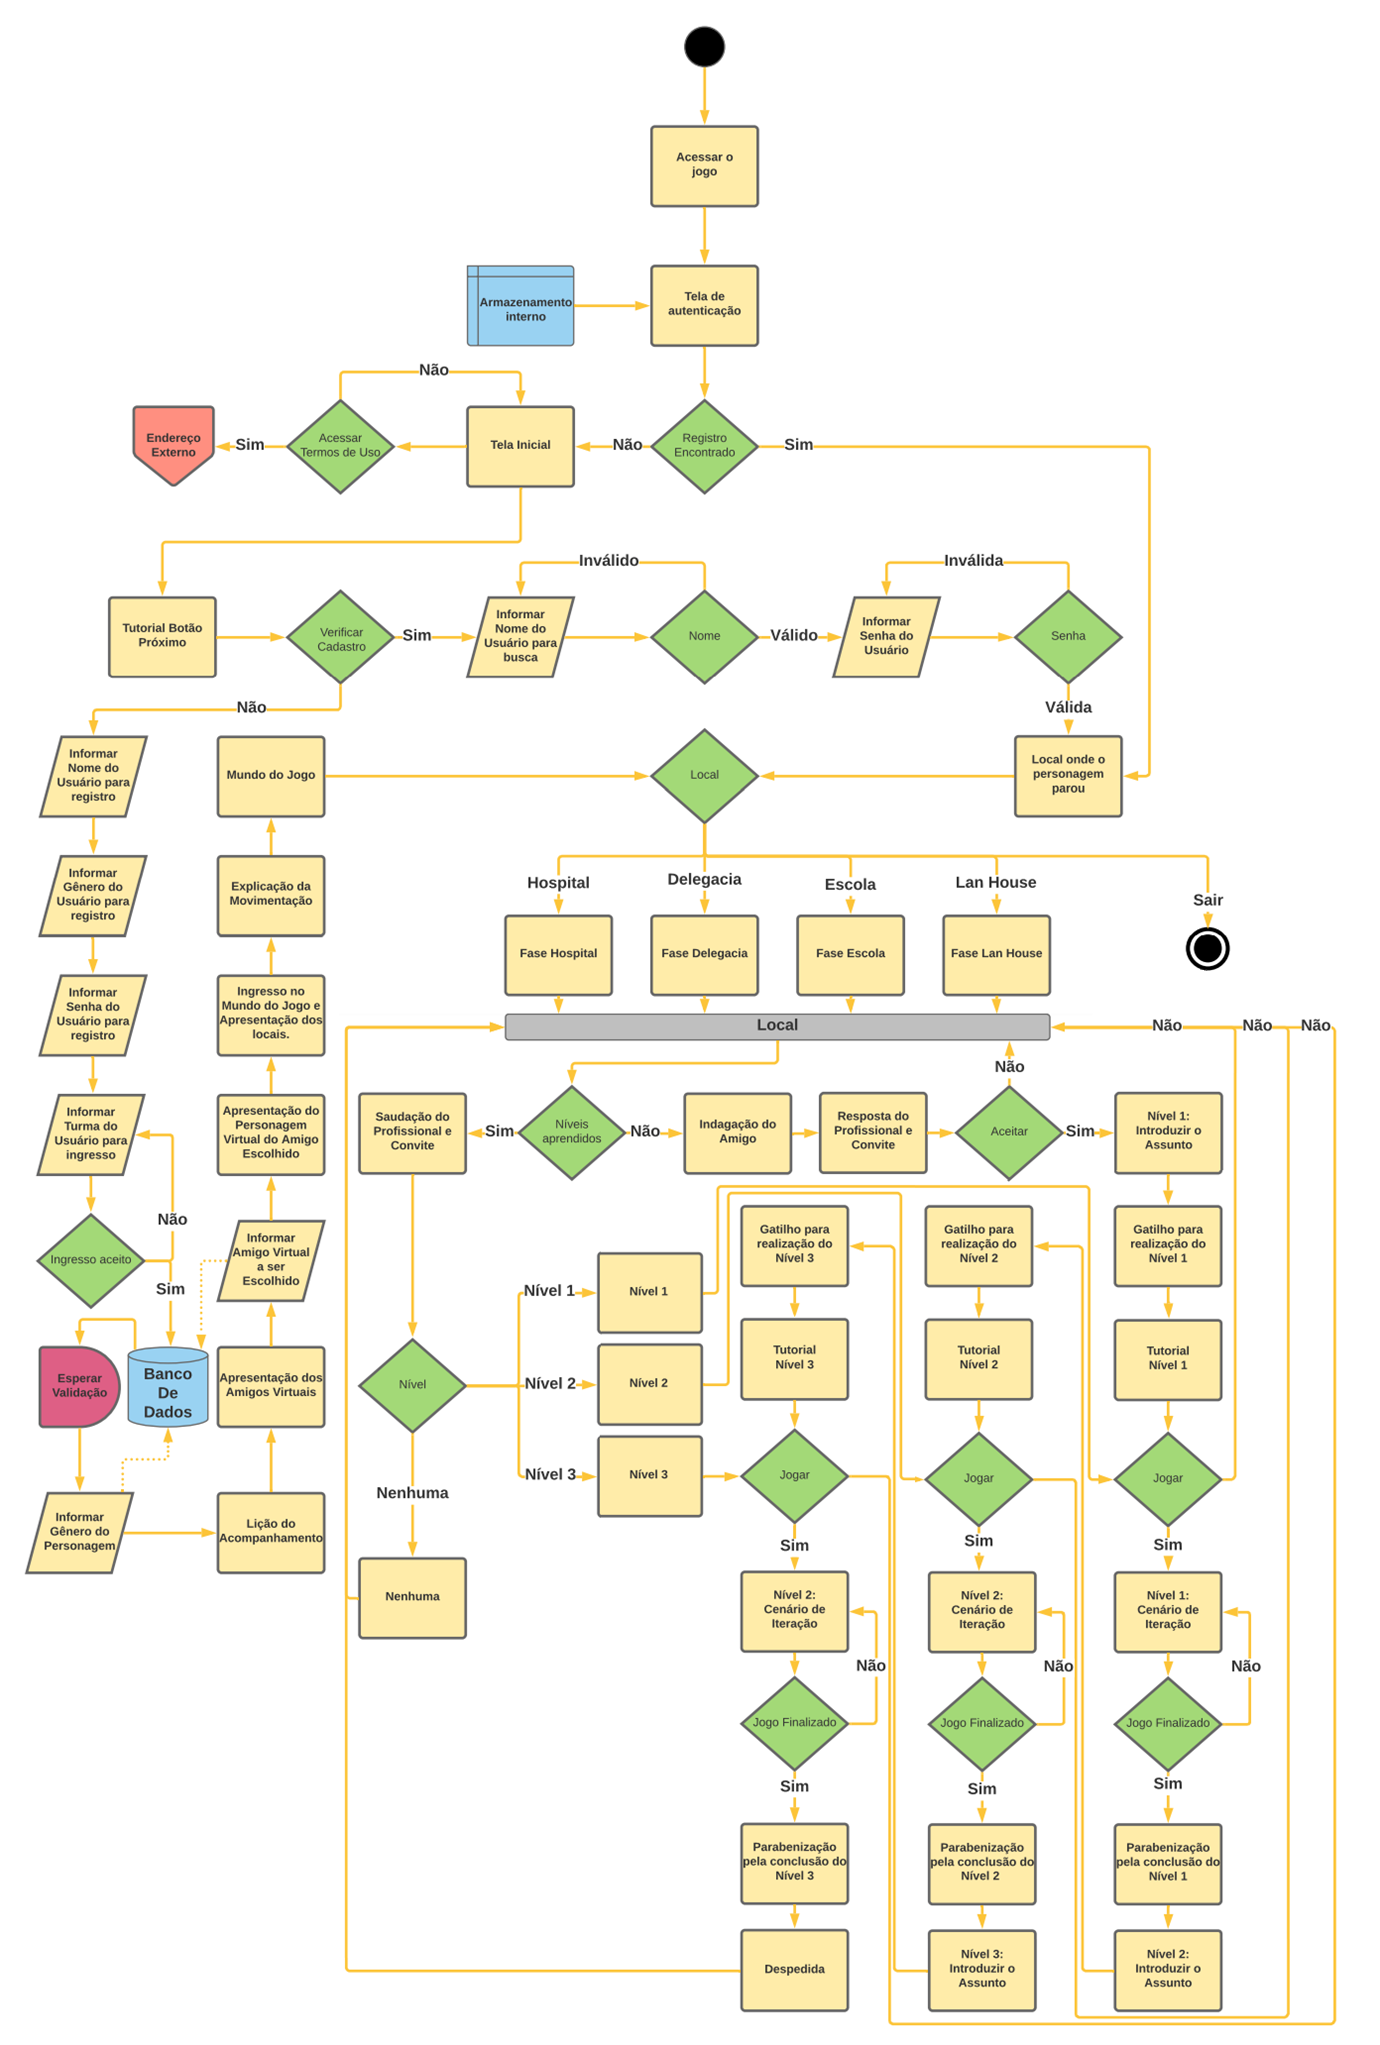
\includegraphics[width=0.95\linewidth]{./Figuras/DiagramaJoginho.png}
  \end{center}\vspace{-0.6cm}
\legend{Fonte: os autores}

\end{figure}


O diagrama de atividades da \autoref{fig:Diagrama}, representa de forma gráfica o fluxo de etapas necessárias para concluir cada atividade do jogo. A parte supeior corresponde as atividades relacionados ao acesso ao jogo. As atividades relacionadas ao cadastro no jogo é representados na parte esquerda do diagrama. Todas as demais atividades representadas no diagramas correspondem ao jogo em si. São quatro fases presentes no jogo: Fase do Hospital, Fase da Delegacia, Fase da Escola e Fase da Lan House. Cada fase possui três nível, em cada nível os jogadores aprendem conteúdos relacionados a prevenção da violência sexual infantil. 

\end{comment}

%O desconforto que imagens realistas poderiam causar no público e que fariam o jogo perder um pouco do caráter divertido. %https://www.sbgames.org/proceedings2020/ArtesDesignFull/209677.pdf (o fluxograma grama deles de ensinamentos é bem legal)

O jogo sério desenvolvido ministra assuntos sensíveis relacionados a sexualidade e a prevenção da violência sexual infantil. Por tal razão, todo o fundamental teórico do jogo advém de documentos devidamente revisados por especialistas na área de educação e sexualidade. Ainda no aspecto pedagógico, salienta-se que o jogo não se utiliza de elementos visualmente realistas. %Ou seja, o jogo não se utliza de artes realistas para apresentar um determinado conceito ou uma determinada situação. 
A literatura relata que a utilização de imagens reais de cunho sexual trazêm desconforto para alguns indivíduos, por tal razão toda a arte utilizada no jogo assume uma ilustração no estilo de um desenho infantil \cite{jogo2020Albert}.



%Jogos sérios devem balançear os aspectos didáticos e lúdicos do jogo. 

%O jogo projetado neste trabalho almeja a prevenção da violência sexual infantil. Embora a educação sexual seja o aspecto de maior presença no jogo, outras questões didático-pedagógicas ainda são levadas em consideração. Visando ajudar no letramento e na alfabetização das crianças, o jogo transcreve todos os diálogos na fonte \textit{Gill Sans}. A fonte \textit{Gill Sans} destaca-se com uma das melhores fontes para o desenvolvimento da leitura infantil \cite{lourencco2011tipografia}. 


%O jogo precisa agradar o público infantil com uma boa jogabilidade e bons desafios, na mesma medida que educa as crianças \cite{valenza2018guidelines}. Entre os aspectos que provocam engajamento do público infantil está a dublagem. No jogo desenvolvido, além da dublagem ser associada ao texto escrito existe a procupação com o letramento e alfabetização infantil. Por tal razão, os dialógos do jogo são escritos na fonte \textit{Gill Sans}.

O jogo sério desta pesquisa possui uma estrutura metodológica de ensino baseada em quatro princípios a serem ministrados: Anatomia (\autoref{subsec:1}), Direitos (\autoref{subsec:2}), Denúncias (\autoref{subsec:3}) e Ciberespaço (\autoref{subsec:4}). Cada um desses princípios se traduzem em uma fase no jogo, cada qual composta de três níveis. A \autoref{fig:conceitos} apresenta cada fase do jogo associada aos seus respectivos níveis.

%\vspace{-0.2cm}

\begin{figure}[hbt!]
  \caption{\label{fig:conceitos}Conceitos abordados}\vspace{-0.2cm}
  \begin{center}
    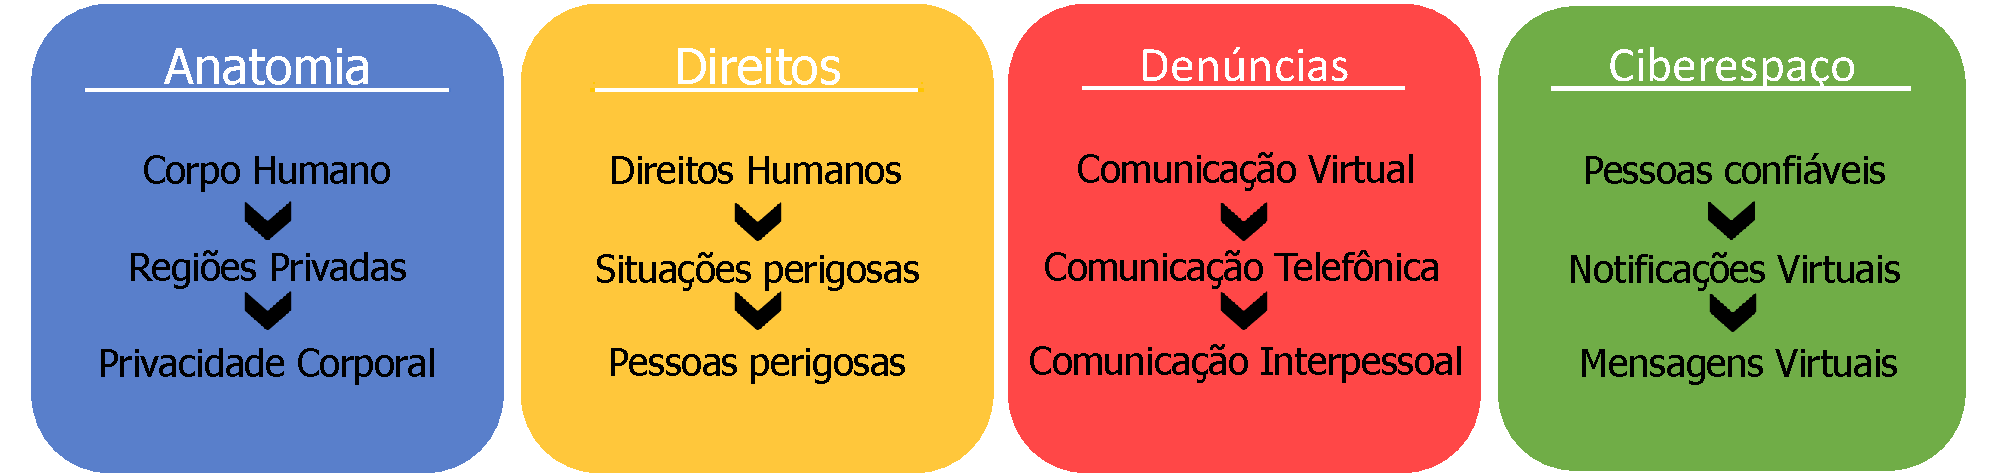
\includegraphics[width=\linewidth]{./Figuras/EsquemaFases.pdf}
    \end{center}\vspace{-0.5cm}
  \legend{Fonte: os autores}
  
\end{figure}

\vspace{-0.2cm}

A \autoref{fig:conceitos} ilustra de maneira resumida cada um dos conteúdos a serem ministrados pelo jogo. Cada conteúdo é ministrado em um ambiente específico do jogo. Ou seja, o jogador possui liberdade de movimentação sobre o jogo, podendo alternar entre as fases da maneira que melhor lhe convir. Respectivamente, os conceitos sobre \textbf{Anatomia} são ministrados em um Hospital. Os direitos das crianças são ensinados em uma \textbf{Escola}. A realização de denúncias é um assunto ensinado em uma \textbf{Delegacia}. E a proteção no ambiente virtual das redes é ministrado em um \textbf{Cibercafé}.

A jogabilidade de jogo é flexível, permitindo ao jogador intercambiar entre as fases sem qualquer punição. Entretanto, os níveis das fases obedecem uma linearidade tanto de enredo, quando pedagógica (e.g. na fase da anatomia o jogador deve necessariamente aprender antes sobre os nomes das partes do corpo, para em seguida aprender quais são as partes íntimas do corpo, para por fim aprender os locais onde as pessoas podem tocar no corpo). O jogador tem liberdade para abandonar um nível sempre que desejar. Contudo, os últimos níveis são alcançáveis apenas após a conclusão dos anteriores. 

\newpage

\subsection{Anatomia}\label{subsec:1}

O jogo desenvolvido apresenta aos jogadores conceitos sobre anatomia em um ambiente hospitalar. Três minijogos buscam ensinar aos jogadores questões sobre o Corpo Humano, Regiões Privadas e Privacidade Corporal. A \autoref{fig:Hospitalzinho} ilustra as dinâmicas utilizadas em cada um dos minijogos. Todos os conceitos desse ambiente são ministrados pelo personagem de um médico. 


\begin{wrapfigure}[25]{r}{6.0cm}%pulando 29 linhas
  \vspace{-20pt}
  \caption{\label{fig:Hospitalzinho}Hospital}
  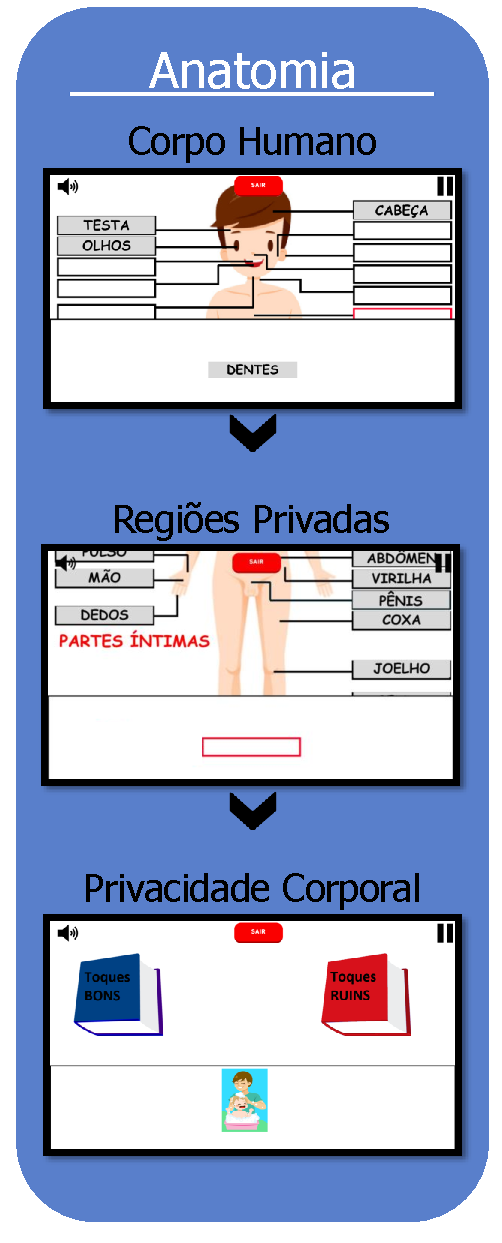
\includegraphics[width=\linewidth]{./Figuras/Hospital.pdf}
  \vspace{-1.0cm}
  \legend{Fonte: os autores}
\end{wrapfigure}

O primeiro minijogo (Corpo Humano) busca ensinar ao jogador o nome correto das partes do corpo humano. Com o auxílio de um mural ilustrativo, o jogador é capaz reconhecer as nomenclaturas corretas corpo humano masculino e feminino. Após um determinado evento, as  algumas peças do mural caem. O jogador deve então, demonstrar seus conhecimentos sobre o corpo humano, inserindo as peças em suas respectivas posições. As peças vão aparecendo uma a uma no centro da caixa de diálogo, sendo que o jogador deve arrastá-las e movê-las para suas posições originais. As peças não encaixam em outras posições que não sejam as originais, nesses casos o jogador é informado sonoramente e visualmente dos seus equívocos. 


O segundo minijogo (Regiões Privadas) busca ensinar ao jogador as partes íntimas do corpo humano. O médico educa o jogador sobre as zonas privadas e não privadas do corpo no mesmo mural do primeiro minijogo. As regiões privadas são representadas por peças com contorno vermelho no mural. Após o jogador ter adquirido esse conhecimento, os contornos vão ao chão. Neste momento o jogador deve levar os contornos vermelhos para as peças que representam as partes íntimas.

O terceiro minijogo (Privacidade Corporal) busca ensinar ao jogador sobre os toques bons e ruins. Neste minijogo são apresentados dois livros, um apenas com imagens de toques bons e outro apenas com imagens de toque ruins. Um dado evento faz com que as imagens se misturem entre os livros. O jogador deve então demonstrar seus conhecimentos classificando devidamente as imagens. As imagens vão aparecendo uma por uma na caixa de diálogo, com o jogador tendo que movê-las para seus respectivos livros. Após esse minijogo, o jogador completa a etapa de Anatomia.% do jogo. 

\subsection{Direitos}\label{subsec:2}

O jogo projetado neste trabalho apresenta aos jogadores seus direitos e deveres. Três minijogos buscam ensinar aos jogadores questões sobre Direitos Humanos, Situações Perigosas e Pessoas Perigosas. A \autoref{fig:Escola} ilustra as dinâmicas utilizadas em cada um dos minijogos. Todos os conceitos desse ambiente são ministrados pela personagem de uma professora. 

\begin{wrapfigure}[25]{r}{6.0cm}%pulando 29 linhas
  \vspace{-20pt}
  \caption{\label{fig:Escola}Escola}
  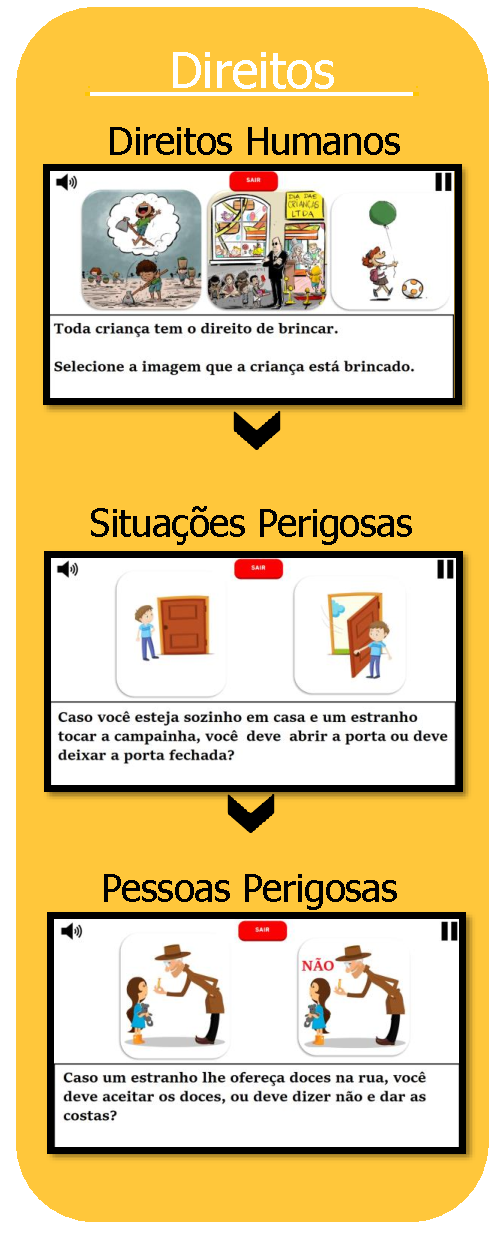
\includegraphics[width=\linewidth]{./Figuras/Escola.pdf}
  \vspace{-1.0cm}
  \legend{Fonte: os autores}
\end{wrapfigure}

O primeiro minijogo (Direitos Humanos) busca ensinar ao jogador sobre os direitos da criança no Brasil e no mundo. O minijogo discorre sobre os direitos e deveres das crianças. Por meio de um jogo de perguntas e respostas com imagens a criança deve associar determinado direito ou dever com uma das imagens apresentadas. O jogador então além de ser ensinado verbalmente e textualmente sobre seus dinheiros, demonstra seus conhecimentos em uma representação visual. Tal método de ensino, demonstra a capacidade de abstração da criança ao criar uma imagem mental dos conceitos aprendidos e associar essa imagem mental a uma imagem no jogo. 

O segundo minijogo (Situações Perigosas) visa educar o jogador sobre sua segurança. O jogador é ensinado que as crianças não estão totalmente protegidas de seus direitos, sendo importante tomar cuidado com determinadas situações que podem colocá-las em risco. %na qual os direitos das crianças seriam desrespeitados. 
Com o auxílio de imagens, um conjunto de situações é apresentado ao jogador onde o jogador deve optar em escolher duas situações. Nesse jogo de perguntas e respostas o jogador deve então demonstrar sua perspcácia em evitar situações potencialmente perigosas.

O terceiro minijogo (Pessoas Perigosas) busca ensinar ao jogador sobre pessoas que podem desrespeitar os direitos das crianças. O minijogo em si realiza uma série de perguntas e respostas similar as do segundo minijogo, porém ao invés de apresentar situações, pessoas são apresentadas. Nesse jogo, o jogador deve então demonstrar sua habilidade em evitar pessoas que apresentem atitudes potencialmente perigosas. Após a conclusão deste minijogo, o jogador finaliza a etapa de Direitos. 

\subsection{Denúncias}\label{subsec:3}

O jogo sério deste trabalho apresenta aos jogadores formas nas quais são possíveis formalizar uma denúncia. Três minijogos buscam ensinar aos jogadores questões relacionadas a Comunicação Virtual, Comunicação Telefônica e Comunicação Interpessoal. A \autoref{fig:DelegaciaDP} ilustra as dinâmicas utilizadas em cada um dos minijogos. Os conceitos desse ambiente são passados pelo personagem de um delegado. 

\begin{wrapfigure}[25]{r}{6.0cm}%pulando 29 linhas
  \vspace{-20pt}
  \caption{\label{fig:DelegaciaDP}Delegacia}
  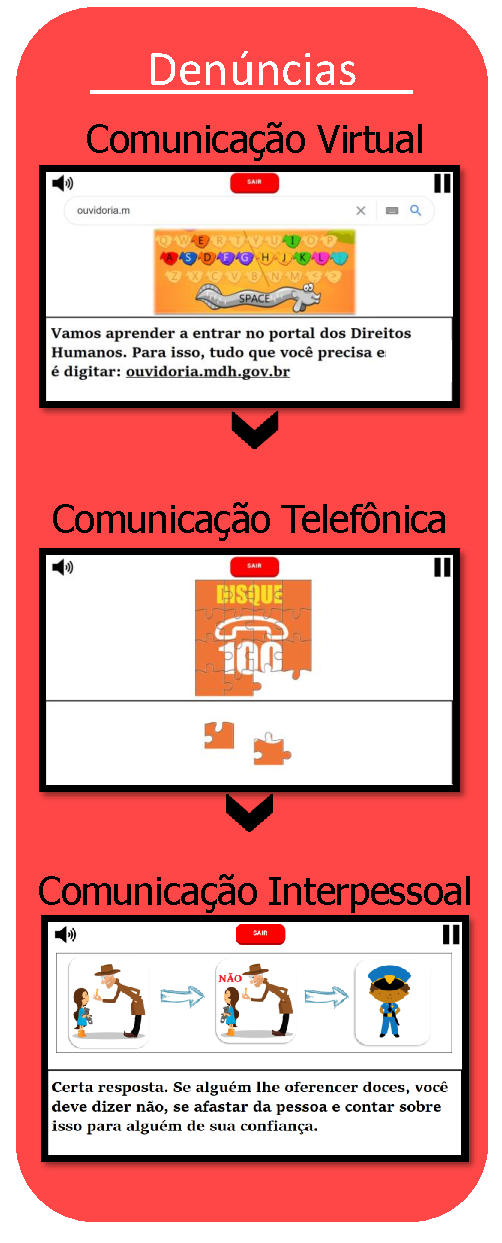
\includegraphics[width=\linewidth]{./Figuras/Delegacia.pdf}
  \vspace{-1.0cm}
  \legend{Fonte: os autores}
\end{wrapfigure}


O primeiro minijogo (Comunicação Virtual) busca apresentar ao jogador as formas virtuais de se realizar uma denúncia no Brasil. Nesse sentido, o minijogo introduz um computador onde um jogo de datilografia se inicia. Nesse jogo, o jogador é instruído a pesquisar e digitar corretamente os canais nacionais de denúncia. O jogo obedece uma estruturo lúdico-pedagócica de forma a ser acessível para as crianças que não encontram-se totalmente alfabetizadas. 

O segundo minijogo (Comunicação Telefônica) ensina ao jogador sobre as linhas telefônicas para a denúncia de crimes contra a criança. Um mural com um número telefônico é apresentado ao jogador. Após o jogador visualizar o mural, um dado evento, faz com que o mural se fragmente. Em um jogo de quebra-cabeça o jogador deve então montar novamente o mural. A dinâmica lúdica utilizada neste jogo, prolonga o contato do jogador com o canal de denúncia do Disque 100, ampliando assim a retenção da informação. Peças colocadas em posições incorretas não provocam sinais sonoros ou visuais de erro. Entranto, peças colocadas em locais corretos ficam fixadas ao mural, impossibilitando de serem movidas novamente. 

O terceiro minijogo (Comunicação Interpessoal) busca ensinar ao jogador como realizar denúncias pessoalmente. Neste minijogo, um livro ilustrado é apresentado ao jogador. As situações ilustradas representam eventos ordenados. Uma dada situações faz com que a ordem das ilustrações seja embaralhada. Neste momento, o jogador é confrontado a montar novamente a ordem dos acontecimentos (eventos) ilustrada no livro. 
%O jogador então demonstra como se comportar em um conjunto de situações e como relatar os acontecimentos para uma pessoa confiável. 
O término deste minijogo, implica na conclusão da etapa de Denúncias. 

\subsection{Ciberespaço}\label{subsec:4}

O jogo desenvolvido elenca maneiras seguraças para as crianças se proteger nas redes. Três minijogos buscam ensinar as crianças questões sobre Pessoas Confiáveis, Notificações Virtuais e Mensagens Virtuais. A \autoref{fig:Cibercafe} ilustra as dinâmicas utilizadas em cada um dos minijogos. Todos os conceitos desse ambiente são ministrados pelo personagem de um robô. 


\begin{wrapfigure}[25]{r}{6.0cm}%pulando 29 linhas
  \vspace{-20pt}
  \caption{\label{fig:Cibercafe}Cibercafé}
  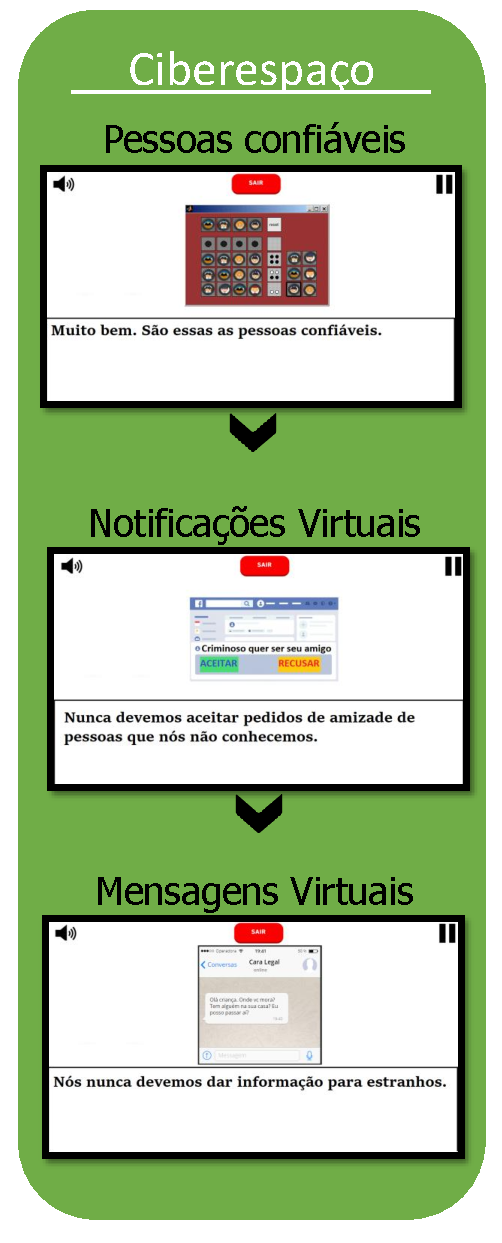
\includegraphics[width=\linewidth]{./Figuras/Cibercafe.pdf}
  \vspace{-1.0cm}
  \legend{Fonte: os autores}
\end{wrapfigure}

O primeiro minijogo (Pessoas Confiáveis) busca ajudar o jogador a identificar pessoas de confiança. Uma situação é apresenta ao jogador neste minijogo, o qual é confrontado a acessar um computador por intermédio de uma senha. A senha em si, compreende um conjunto de fotos dos personagens confiáveis que o jogador encontrou durante o jogo. A dinâmica deste minijogo consiste na tentativa e erro do jogador em montar um conjunto de pessoas de confiança até atingir a combinação correta. Durante esse minijogo as escolhas certa e erradas são justificadas ao jogador, ajudando a compreender o que define uma pessoa de confiança ou não. 

O segundo minijogo (Notificações Virtuais) busca ensinar ao jogador como se comportar nas redes sociais. O minijogo enfatiza da importância das redes sociais e salienta que crianças menores de 13 anos não deveriam usar redes como o \textit{Facebook}. Contudo, caso usem, o jogo reforça a necessidade e o cuidado em adicionar apenas pessoas conhecidas e também avisa sobre a existência de perfis falsos se passando por pessoas conhecidas. A dinâmica deste minijogo consiste no jogador aceitar e recursar devidamente pedidos de amizade, além de aprender a desfazer amizades. %(caso um erro seja cometido). 

O terceiro minijogo (Mensagens Virtuais) ensina ao jogador como se comunicar nas redes. O minijogo explica que alguns serviços de mensagem instantânea como o \textit{Whatsapp} também possuem uma idade mínima para uso (13 anos de idade), porém diferente do \textit{Facebook}, qualquer pessoa é capaz de enviar mensagens sem a prévia autorização da outra pessoa. A dinâmica do jogo consiste em ensinar o jogador a não compartilhar informações com estranhos e relatar os acontecimentos para um adulto de confiança. Após esse minijogo, o jogador completa a etapa de Ciberespaço. 

% A dinâmica do jogo consiste em ensinar o jogador a não compartilhar informações com estranhos, além de bloqueá-los e relatar os acontecimentos para um adulto de confiança. Após esse minijogo, o jogador completa a etapa de Ciberespaço. 


\begin{comment}
propósito

Orientações em Sexualidade

Plataforma

Publico Alvo

Estilo

Estética

Arte

Fonte

Escalabilidade/Flexibilidade

Audio

Musica

Leiaute de Níveis

UX

Gamificação

Ergonomia de Botões

Artefato

Licença

Termos de Serviço

Política de Privacidade

Criptografia

Banco de Dados
\end{comment}

\section{Considerações Finais}\label{sec:fim}

O jogo sério projetado por este trabalho é constituído por doze minijogos voltados a educar os jogadores sobre questões relacionadas a temática da violência sexual infantil. Todos os minijogos, independentemente de sua fase, apresentam a mesma Barra de Estado, como pode ser observado nas telas do jogo das Figuras \ref{fig:Hospitalzinho}, \ref{fig:Escola}, \ref{fig:DelegaciaDP} e \ref{fig:Cibercafe}. A Barra de Estado (HUD - Head-Up Display), é uma região da tela do jogador na qual informações ou elementos são dispostos de modo a não atrapalhar a visão do jogador, sendo anexados normalmente nas extremidades da tela. Os elementos da Barra de Estado do jogo são um botão para silenciar/desilenciar o jogo (canto superior direito), um botão para parar/desparar o jogo e um botão vermelho para sair dos minijogos (centro superior). O botão vermelho situado na região superior de todos os doze minijogos é um botão presente apenas nestes momentos. Quando o jogador está transitando entre os ambientes do jogo, o botão não é apresentado. 

%pois para sair do jogo como um todo, o jogador precisa apenas encerra a aplicação. No entanto, para sair dos minijogos, basta apenas clicar no botão vermelho.

Todas as ações realizadas pelos jogadores durante as dinâmicas ministradas no jogo são enviadas para um banco de dados relacional. Dados sobre a quantidade de acertos e erros preenchem os campos no banco de cada um dos jogadores. Os dados gerados pelo sistema não são apresentados ao jogador em nenhum momento. As informações coletadas servem para compreender melhor o desempenho dos jogadores e suas preferências. O jogo opera unicamente em navegadores, necessitando de uma conexão via servidor para ser carregado no navegador. A conexão via servidor ainda se faz necessária durante os minijogos, pois são durante estes momentos que o jogo realiza requisições ao banco de dados. 

%O jogo desenvolvido encontra-se hospedado publicamente. Salienta-se nesse sentido que até a data de publicação deste trabalho a corrente versão do jogo encontra-se inacabada. Desta forma, não se recomenda que o jogo seja ministrado para crianças até a formulação de uma versão mais robusta e acabada do jogo. Sua disponibilização ao público objetiva-se apenas em uma publicação mais detalhada dos frutos da presente pesquisa. Dito isso, o jogo em questão encontra-se hospedado na plataforma de desenvolvimento de aplicativos para dispositivos móveis \textit{Firebase} da empresa multinacional de serviços \textit{Google}, sendo acessível pelo seguinte endereço da \textit{internet}: \url{https://infancia.firebaseapp.com/}

Grande parte dos minijogos estão em acordo com conceitos recomendados pelas orientações técnicas internacionais de educação em sexualidade \cite{women2018international}. Os únicos dois minijogos que não encontram-se em harmônia com as orientações internacionais são os conceitos de \textbf{Comunicação Virtual} e \textbf{Comunicação Telefônica}. A introdução destes dois conceitos ao jogo, surge como uma medida de fortaceler as estratégias e campanhas nacionais de concientização infantil. O estudo bibliográfico do presente trabalho identificou medidas nacionais focadas na divulgação dos ramais e canais de denúncia dos direitos das crianças. Almejando a divulgação de tais canais, optou-se em anexar, os dois conceitos citados, ao jogo. Com exceção deste conceitos, todos os demais assuntos estão em consonância com as orientações da \citeonline{women2018international}. Diante do exposto, enfatiza-se que o jogo sério desenvolvido por este trabalho baseia seus ensinamentos em conceitos didáticos reconhecidos na área em questão. Assim como, baseia seus processo de desenvolvimento em aspectos técnicos reconhecidos no campo de  desenvolvimento de jogos. O próximo passo da corrente pesquisa, consiste na realização de testes com usuários para se verificar a eficácia, ou não, do jogo no que tange o combate a violência sexual infantil. 






%O  minijogo \textbf{Corpo Humano} está associado a parte dos conceitos de anatomia da UNESCO. Os minijogos \textbf{Regiões Privadas} e \textbf{Privacidade Corporal} se relacionam com os conceitos de consentimento, privacidade e integridade corporal da UNESCO. O minijogo \textbf{Direitos Humanos} remete ao tópico direitos humanos das orientações técnicas da UNESCO. Os minijogos \textbf{Situações Perigosas} e \textbf{Pessoas Perigosas} se relacionam com os tópicos de violência e tomada de decisões. O minijogo \textbf{Comunicação Interpessoal} remete as questões sobre encontrar ajuda e apoio da UNESCO, assim como o minijogo \textbf{Pessoas Confiáveis}. Por fim, os minijogos \textbf{Notificações Virtuais} e \textbf{Mensagens Virtuais} abordam sobre assuntos relacionados a utilização segura das TIC como orienta a UNESCO. 






%%%%%%%%%%O enredo é tão importante para jogos sérios como não-sérios, pois permite que o jogador se projete na personagem do jogo (McDaniel et al., 2010). [tese Adilson] = Falar da dinâmica do herói mudo.


%Digital Natives. Our students today are all “native speakers” of the digital language of computers, video games and the Internet. %https://www.marcprensky.com/writing/Prensky%20-%20Digital%20Natives,%20Digital%20Immigrants%20-%20Part1.pdf %https://colegiongeracao.com.br/novageracao/2_intencoes/nativos.pdf


%Para que um game seja completo, e atenda a critérios de usabilidade, é essencial promover algum mecanismo que facilite o aprendizado do funcionamento do jogo. De acordo com Squire et al. (2005, p.41), mediadores são fundamentais nos primeiros dias%https://www.udesc.br/arquivos/cct/id_cpmenu/1024/diego_buchinger__1__15167055468902_1024.pdf


%A Metodologia Institucional “Aprender na Prática”, que prevê “a ação educativa na participação ativa e crítica do aluno em sua aquisição de conhecimentos práticos e teóricos” [UNICSUL, 2004] 


%desenvolvimento solitário baseado em ambiarra (DSBA)